\part{Wissensrepräsentation und lineare kontinuierliche Systeme}
\section{Lineare kontinuierliche Systeme}
\subsection{Welche Annahmen liegen dem linearen Einspurmodell zugrunde? Nennen Sie mindestens 5 Stück.}
\subsection{Zeichnen Sie ein Blockschaltbild eines dynamischen Systems mit Beobachter. Beschriften Sie das
    Blockschaltbild sorgfältig.}
\subsection{Reduzieren Sie das gegebene Querführungsmodell 5.Ordnung soweit wie möglich, so dass damit ein
    Schwimmwinkelbeobachter konstruierbar ist. Notieren Sie das Modell in Zustandsdarstellung unter der
    Annahme, dass der Lenkwinkel die einzige Eingangsgröße ist.}
\begin{equation}
    \left(
    \begin{array}{c}
            \dot{\lambda}    \\
            \ddot{\Psi_V}    \\
            \dot{\beta}      \\
            \dot{\Psi_{rel}} \\
            \dot{y}          \\
        \end{array}
    \right)=
    \left(
    \begin{array}{ccccc}
            0                                & 0                                                        & 0                                                   & 0 & 0 \\
            \dfrac{c_{\alpha v}l_{v}}{I_{z}} & -\dfrac{c_{\alpha v}l_{v}^2+c_{\alpha h}l_{h}^2}{I_{z}v} & -\dfrac{c_{\alpha v}l_{v}-c_{\alpha h}l_{h}}{I_{z}} & 0 & 0 \\
            \dfrac{c_{\alpha v}}{mv}         & -1-\dfrac{c_{\alpha v}l_{v}-c_{\alpha h}l_{h}}{mv^2}     & -\dfrac{c_{\alpha v}+c_{\alpha h}}{mv}              & 0 & 0 \\
            0                                & 1                                                        & 0                                                   & 0 & 0 \\
            0                                & 0                                                        & v                                                   & v & 0 \\
        \end{array}
    \right)
    \left(
    \begin{array}{c}
            \lambda      \\
            \dot{\Psi_V} \\
            \beta        \\
            \Psi_{rel}   \\
            y            \\
        \end{array}
    \right)+
    \left(
    \begin{array}{c}
            1 \\
            0 \\
            0 \\
            0 \\
            0 \\
        \end{array}
    \right)\dot{\lambda}+
    \left(
    \begin{array}{c}
            0  \\
            0  \\
            0  \\
            -v \\
            0  \\
        \end{array}
    \right)c_0
\end{equation}
\subsection{Beschriften Sie folgende schematische Darstellung des linearen Einspurmodells in der nachstehenden Tabelle.}
\begin{figure}[H]
    \begin{minipage}[c]{.45\linewidth}
        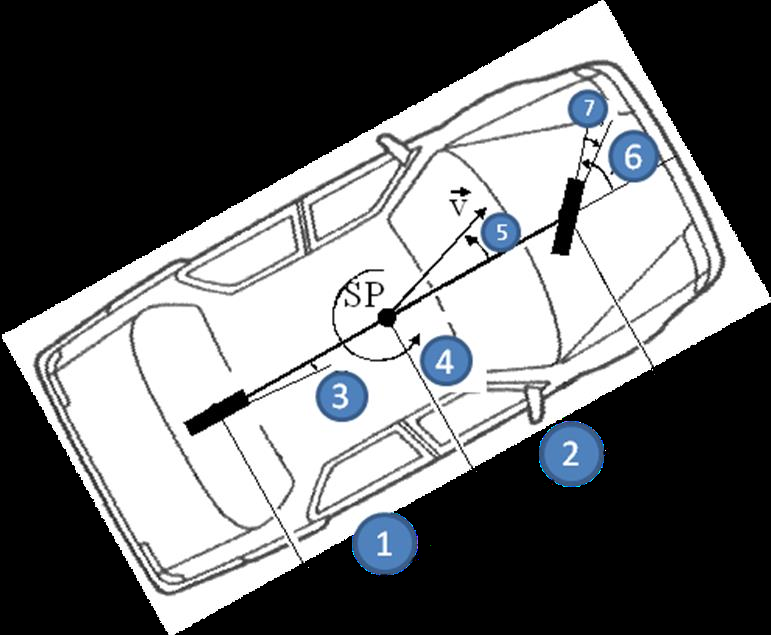
\includegraphics[width=\linewidth]{Graphics/Linearen_Einspurmodell.png}
    \end{minipage}
    \begin{minipage}[c]{.45\linewidth}
        \begin{tabular}{|p{.2\linewidth}|p{.4\linewidth}|p{.4\linewidth}|}
            \hline
            Nr.&Bezeichnung&Bedeutung\\
            \hline
            1& & \\
            \hline
            2& & \\
            \hline
            3& & \\
            \hline
            4& & \\
            \hline
            5& & \\
            \hline
            6& & \\
            \hline
            7& & \\
            \hline
        \end{tabular}
    \end{minipage}
\end{figure}
\subsection{Beobachter}
\subsubsection{Wo liegen die Pole der Übertragungsmatrix eines Beobachters in Abhängigkeit von der Rückführungsmatrix
L? Geben Sie eine Herleitung für Ihr Ergebnis an.}
\subsubsection{}
Für folgendes System soll ein Beobachter zur Zustandsrekonstruktion so entworfen werden, dass
die Beobachterfehlerdynamik einen doppelten Pol bei $s=-2$ aufweist.
\begin{equation}
    \begin{array}{l}
        \dot{x}=\left[\begin{array}{cc}
            2&1\\
            -1&0\\
        \end{array}\right]x+\left[\begin{array}{c}
            0\\
            1\\
        \end{array}\right]u\\
        y=\left[1\qquad 0\right]x
    \end{array}
\end{equation}
\paragraph{1.Überprüfen Sie das System auf die Beobachtbarkeit.
}
\paragraph{2. Bestimmen Sie die Beobachterkoeffizienten und .
}